\parindent=0em
\documentclass[11pt, oneside]{article}   						%use article, report, book

%% !TEX TS-program = latex
%%Vorspann von Ulla Aeschbacher%%
%-----------------------------------------------------------------------------------------------------------------------------------------------------------------------
\usepackage[paper=a4paper,left=27mm,right=27mm,top=30mm,bottom=30mm]{geometry} 	                        	%für Seitenränder und vieles weitere

\usepackage{tikz}												                        		            %tikzpicture
\usetikzlibrary{arrows.meta}									                        	              	%arrowheads length and width
\usetikzlibrary{calc}
\usetikzlibrary{decorations.text}
\usetikzlibrary{decorations.pathmorphing}
\usepackage{pgfplots}                                                                                       %for easily adding plots
\pgfplotsset{compat=1.15}

\usepackage{amsmath}									                        		            		%For multiline equations
\usepackage{ifsym}
\usepackage{amssymb}									                         		            		%For mathbb
\usepackage{mathtools}										                        	            		%For matrices and writing over arrows
\usepackage{bm}												                                       		    %To write bold in math mode
\usepackage{extpfeil}										                                      			%For more varieties in arrows 
\usepackage{extarrows}									            				                        %For long text over long arrows
    
\usepackage{amsthm}										            			                            %For not cursive theorems
\usepackage{framed}										            	                        		    %for frames around theorems
\usepackage{thmtools}											                                    		%for easy custom theorems

\usepackage{enumerate}										                                     			%To be able to customize \benum[a)] \benum[**(i)**] etc...
\usepackage{chngcntr}                                                                                       %to enumerate theorems within section,subsection etc.

\usepackage[parfill]{parskip}									                                       		%no indentation for paragraphs

\usepackage{color}											                                    			%to color text
\usepackage{multicol}										                                    			%use as \begin{multicol}
\usepackage{multirow}									                                    				%for multirow/multicolumn in tabular
\usepackage{caption} 									                                    				%captions for pictures in 
\usepackage{newfloat}
    %for defining new floats
 
\usepackage{listings}									                                    				%for code

\usepackage{algorithm}								                                    					%for algorithms
\usepackage{algpseudocode}							                                    					%from algorithmicx, for creating new blocks
\usepackage{float}									                                    					%use [H] after floating environments to fix placement

\clubpenalty=10000								                                    						%für Hurenkinder und Schusterjungen	
\widowpenalty=10000
%-----------------------------------------------------------------------------------------------------------------------------------------------------------------------
\definecolor{mred}{rgb}{0.82, 0.1, 0.26}
\definecolor{mblue}{rgb}{0.0, 0.73, 0.84}
\definecolor{mgreen}{rgb}{0.0, 0.8, 0.0}
\newcommand{\tr}[1]{\textcolor{mred}{#1}}
\newcommand{\tb}[1]{\textcolor{mblue}{#1}}
\newcommand{\tg}[1]{\textcolor{mgreen}{#1}}
%-----------------------------------------------------------------------------------------------------------------------------------------------------------------------
%   \begin{mydef}[Degree] The number of neigbors of a vertex. \end{mydef}
%	Definition 1 Degree: The number of neigbors of a vertex.
\makeatletter
\declaretheoremstyle[
	spaceabove=6pt, spacebelow=6pt,
	headfont=\normalfont\bfseries,
	notefont=\color{mgreen}\bfseries, 
	notebraces={}{},
	bodyfont=\normalfont,
	postheadspace=0.5 em,
	headpunct={:},
	spacebelow=\parsep,
    	spaceabove=\parsep,
	postheadhook={%
		\ifx\@empty\thmt@shortoptarg
		\renewcommand\addcontentsline[3]{}
		\fi},
]{mydef}
\declaretheorem[name={Definition}, style=mydef]{mydef}
\makeatother

%   \begin{mythm}[Gauss] The number of neigbors of a vertex. \end{mythm}
%	\box{Theorem 1 (Gauss): The number of neigbors of a vertex.}
\makeatletter
\declaretheoremstyle[
	spaceabove=6pt, spacebelow=6pt,
	headfont=\normalfont\bfseries,
	notefont=\color{mred}\bfseries, 
	notebraces={}{},
	bodyfont=\normalfont,
	postheadspace=0.5 em,
	headpunct={:},
	spacebelow=\parsep,
    	spaceabove=\parsep,
	postheadhook={%
		\ifx\@empty\thmt@shortoptarg
		\renewcommand\addcontentsline[3]{}
		\fi},
	mdframed={
		linecolor=black, 
		innertopmargin=6pt,
		innerbottommargin=6pt, 
		skipabove=\parsep, 
		skipbelow=\parsep } 
]{mythm}
\declaretheorem[name={Theorem}, style=mythm]{mythm}
\makeatother

%   \begin{mytitle}[Title] This is the text. \end{mytitle}
%	1 Title: This is the text.
\makeatletter
\declaretheoremstyle[
	spaceabove=6pt, spacebelow=6pt,
	headfont=\normalfont\bfseries,
	notefont=\color{black}\bfseries, 
	notebraces={}{},
	bodyfont=\normalfont,
	postheadspace=0.5 em,
	headpunct={:},
	spacebelow=\parsep,
    	spaceabove=\parsep,
	postheadhook={%
		\ifx\@empty\thmt@shortoptarg
		\renewcommand\addcontentsline[3]{}
		\fi},
	numberwithin=subsection,
]{mytitle}
\declaretheorem[name={}, style=mytitle]{mytitle}
\makeatother

%   \begin{mysubtitle}[Subtitle] This is the text. \end{mysubtitle}
%	1 Subtitle: This is the text.
\makeatletter
\declaretheoremstyle[
	spaceabove=6pt, spacebelow=6pt,
	headfont=\normalfont\bfseries,
	headindent=2em,
	notefont=\color{black}\bfseries, 
	notebraces={}{},
	bodyfont=\normalfont,
	postheadspace=0.5 em,
	headpunct={:},
	spacebelow=\parsep,
    	spaceabove=\parsep,
	postheadhook={%
		\ifx\@empty\thmt@shortoptarg
		\renewcommand\addcontentsline[3]{}
		\fi},
	numberwithin=mytitle,
]{mysubtitle}
\declaretheorem[name={}, style=mysubtitle]{mysubtitle}
\makeatother

%   \begin{myremark} This is the text. \end{myremark}
%	1 : This is the text.
\makeatletter
\declaretheoremstyle[
	spaceabove=6pt, spacebelow=6pt,
	headfont=\normalfont\bfseries,
	notefont=\color{black}\bfseries, 
	notebraces={}{},
	bodyfont=\normalfont\itshape,
	postheadspace=0.5 em,
	headpunct={},
	spacebelow=\parsep,
    	spaceabove=\parsep,
	postheadhook={%
		\ifx\@empty\thmt@shortoptarg
		\renewcommand\addcontentsline[3]{}
		\fi},
	numberwithin=subsection,
]{myremark}
\declaretheorem[name={}, style=myremark]{myremark}
\makeatother

%	\bem{The number of neigbors of a vertex.}
%	Remark 1: \italic{The number of neigbors of a vertex.}
\newtheoremstyle{bemdef}{1em}{1em}{\itshape}{}{\bfseries}{:}{0.5em}{}
\theoremstyle{bemdef}
\newtheorem{bemerkung}{Remark}
\newcommand{\bem}[1]{\begin{bemerkung}#1\end{bemerkung}}
%-----------------------------------------------------------------------------------------------------------------------------------------------------------------------
\newcommand\Tstrut{\rule{0pt}{2.6ex}}        									                            % = `top' strut = Abstand vor /hline in array und tabular
\newcommand\Bstrut{\rule[-0.9ex]{0pt}{0pt}}   									                            % = `bottom' strut = Abstand nach /hline in array und tabular

\iffalse
%use like this
\begin{tabular}{l l}
A & B\\
\hline
a & b\Tstrut\\[0.5em]
c & d\\[0.5em]
e & f
\end{tabular}
\fi
%-----------------------------------------------------------------------------------------------------------------------------------------------------------------------
\newcommand{\vekt}[2]{\left(\begin{array}{r r} #1 \\ #2 \end{array}\right)}						            %2-dim Vektor
\newcommand{\vekts}[2]{\left(\begin{smallmatrix} #1\\ #2 \end{smallmatrix}\right)}				            %small Vektor für in-text
\newcommand{\vek}[3]{\left(\begin{array}{r r r} #1 \\ #2 \\ #3 \end{array}\right)}				        	%3-dim Vektor
\newcommand{\vekb}[3]{\left(\begin{array}{r r r} #1 \\[0.3em] #2 \\[0.3em] #3 \end{array}\right)}		    %3-dim Vektor für Brüche
\newcommand{\vekc}[3]{\left(\begin{array}{c c c} #1 \\ #2 \\ #3 \end{array}\right)}                         %zentrierter 3-dim Vektor
\newcommand{\vekbc}[3]{\left(\begin{array}{c c c} #1 \\[0.8em] #2 \\[0.8em] #3 \end{array}\right)}	        %zentrierter 3-dim Vektor für Brüche
\newcommand{\veks}[3]{\left(\begin{smallmatrix} #1\\ #2 \\ #3 \end{smallmatrix}\right)}			            %small Vektor für in-text
\newcommand{\vekk}[4]{\left(\begin{array}{r r r r} #1 \\ #2 \\ #3 \\ #4 \end{array}\right)}			        %4-dim Vektor
\newcommand{\vekks}[4]{\left(\begin{smallmatrix} #1\\ #2 \\ #3 \\ #4 \end{smallmatrix}\right)}		        %small Vektor für in-text
\newcommand{\efrac}[1]{\frac{1}{#1}}												                        %1/x Bruch
%-----------------------------------------------------------------------------------------------------------------------------------------------------------------------
\newcommand{\doubleu}[1]{\underline{\underline{#1}}}							                            %to double underline something in math mode
%-----------------------------------------------------------------------------------------------------------------------------------------------------------------------
\newcommand{\mc}[1]{\mathcal{#1}}											                                %Mathcal

\newcommand{\mb}[1]{\mathbb{#1}}											                                %Mathbb

\newcommand{\ttt}[1]{\texttt{#1}}											                                %Texttt
%-----------------------------------------------------------------------------------------------------------------------------------------------------------------------
\newcommand{\spr}[2]{\left\langle #1,#2 \right\rangle}							                            %Skalarprodukt
\newcommand{\norm}[1]{\left\Vert #1 \right\Vert}								                            %Norm
\newcommand{\abs}[1]{\left\vert #1 \right\vert}									                            %Betrag
%-----------------------------------------------------------------------------------------------------------------------------------------------------------------------
\newcommand{\rank}{\text{rank}}											                                    %rank
\newcommand{\spann}{\text{span}}											                                %span
\newcommand{\im}{\text{Im}}												                                    %Im
\newcommand{\sign}{\text{sign}}										                                    	%sign
\newcommand{\id}{\text{id }}												                                %id
\newcommand{\diag}{\text{diag}}											                                    %diag
\renewcommand{\ker}{\text{ker}}											                                    %ker
\renewcommand{\dim}{\text{dim}}											                                    %dim
%-----------------------------------------------------------------------------------------------------------------------------------------------------------------------

\tikzset{>=stealth}
\usetikzlibrary{shapes.misc}
\usepackage{marvosym}
\usepackage{stmaryrd} % for \lightning
\usepackage{tabu} % to use X in tabular arguments
\definecolor{firstAccent}{rgb}{1,0.5,0}
\definecolor{secondAccent}{rgb}{1,0,0}
\definecolor{thirdAccent}{rgb}{1,1,0}

\title{Ubiquitous Computing Summary}
\author{Ulla Aeschbacher}
\date{9.7.19} % started, did 1, 2, 3
\date{10.7.19} % did 4, 6
\date{11.7.19} % did 5, 7, 8, 9
\date{2.8.19} % did some typo-fixing and clarifications
\date{5.8.19} % added some more content and graphics

\begin{document}
\maketitle
\tableofcontents

\section{Introduction}
\begin{mytitle}[Ubiquitous computing] Ubiquitous computing is a vision of how we will live and interact with future computing environments. Examples include network embedded systems, wireless sensor networks, wireless communications, distributed systems, mobile devices and human-computer interaction.
\end{mytitle}
\section{Vision}
\begin{myremark}Technical visions slowly become true because of cheaper hardware, smaller hardware, wireless communication at almost no cost and sensors that provide context to objects.
\end{myremark}
\begin{mytitle}[Technological push and application pull] The technological push is complemented by an application pull because there is value for business, society and individuals.
\end{mytitle}
\begin{mytitle}[The evolution of networking]\hfill
\begin{itemize}
    \item Internet: network of computers, TCP/IP
    \item Web: network of documents, HTTP, HTML
    \item network of services, XML, WSDL
    \item network of smart things, JSON
\end{itemize}
\end{mytitle}
\begin{mytitle}[Smart objects] Smart objects are small, cheap and integrated sensors and processors with wireless communication.
\end{mytitle}
\begin{mytitle}[Bits vs. atoms] Bits implement all the smart behaviour, while atoms are the physical objects.
\end{mytitle}
\begin{mytitle}[Technological paternalism] Paternalism can be considered repressive, by protecting people and satisfying their needs but without allowing them any freedom or responsibility. Technological paternalism is already observed today, for example the beeps in a car if the seatbelt is not fastened. The list of potential examples is growing.
\end{mytitle}

\section{Four Ubicomp Drivers}

\subsection{Moore's Law}
\begin{mytitle}[Moore's law] Processing speed and storage capacity doubles around every 18 months.
\end{mytitle}
\begin{mytitle}[Generalized Moore's law] The most important technology parameters like computation cycles, capacity of memory and bandwidth double every 1-3 years. But batteries and users mind-share do not. 
\end{mytitle}
\begin{mytitle}[Batteries] The efficiency of battery technology is improving only slowly over time. Considerations to take into account in respect to batteries include size, weight, cost, peak current vs. average current, rechargable vs. disposable, time to recharge, cycle life and ecological concerns. To save and gain energy we can enable power management in hardware units (shut down unused sections, reduce clock frequency and reduce voltage), use power-aware algorithms and harvest energy from the human body or the environment.
\end{mytitle}

\subsection{New Materials}
\begin{mytitle}[New materials] Examples of new materials are organic semiconductors, flexible displays and graphene. 
\end{mytitle}

\subsection{Progress in Communication Technologies}
\begin{mytitle}[Progress in communication technologies] Examples of new technologies are fiber optics, wireless 5G and bluetooth.
\end{mytitle}
\begin{mytitle}[Near-field communication (NFC)] NFC is short-range (\textasciitilde 10 cm) interaction with handheld devices for example contactless payment. There are many advantages like using almost no energy, requiring only small transmitters and receivers, cheapness, security and no addressing or routing needed.
\end{mytitle}
\begin{mytitle}[Intrabody communication] Intrabody communication works by sending low-power electrical signals through the human body. This allows wearable devices to communicate and enables touch-selective communication. Some applications are that a car can recognize the driver, a shared device configures itself when being touched, devices identifying users and granting access and micro payments. Issues are the fear of phone radiation, safety concerns, reliability and security.
\end{mytitle}

\subsection{Better Sensors}
\begin{mytitle}[Better sensors] Examples of better sensors are miniaturized camers and microphones, biometric sensors, temperature and humidity sensors, acceleration sensors and location sensors.
\end{mytitle}
\begin{myremark} Sensors are the interface between the real world and the cyber space.
\end{myremark}
\begin{mytitle}[Surface acoustic wave (SAW) based sensors] SAW based sensors need no battery or external power supply, they are powered by external RF interrogation signals or alternatively by physical actuation processes. They reflect the RF signal transmitted by an antenna up to 50 m away. The surface wave is a mechanical wave that propagates on the surface of a body, for example on piezo crystals at around 3500 m/s. The transducer then converts electric energy from the RF waves to the surface acoustic wave. Each reflector then sends back parts of the wave. The wave is then transformed back into an RF pulse sequence by the transducer and sent out. The surface wave is much slower than the RF wave, so a response takes more than 2 $\mu$s.
\end{mytitle}
\begin{mytitle}[Applications]
    \begin{mysubtitle}[Applications for SAW] Some applications of SAW are temperature sensors, gas sensors, biosensors and tire sensors.
    \end{mysubtitle}
    \begin{mysubtitle}[Applications for battery-free sensors with transponders] Some applications are identification, temperature sensing, pressure sensing, transport monitoring, product tracking and material flow.
    \end{mysubtitle}
\end{mytitle}


\section[NFC \& RFID]{Near Field Communication (NFC) \& Radio Frequency Identification (RFID)}
\begin{mytitle}[RFID] RFID identifies objects from a distance. It is a small integrated circuit with a radio frequency transponder. A transponder is a transmitter-responder which generates a response to a received signal. The RFID circuit runs on a wireless energy supply due to a magnetic or electromagnetic field. It contains around 100 Bytes of ROM or EEPROM and costs around 1 cent.
\end{mytitle}
\begin{mytitle}[Performance of RFID chips]\hfill
\begin{itemize}
    \item Low end features: read-only memory, tag repeatedly sends out serial number, no collision detection
    \item Medium range features: read-write memory, collision detection
    \item High end features: complex functions such as cryptography
\end{itemize}
\end{mytitle}
\begin{mytitle}[Electronic product tag (EPC)] The EPC is a standard for logistics and retail applications, managed by an industry consortium. It is a unique identifier for finding information providers about a specific product instance.
\end{mytitle}
\begin{mytitle}[Defining features of RFID] RFID systems have four defining features: power supply; operation frequency; communication, coding and modulation, and anti-collision protocols.
\end{mytitle}

\subsection{Power Supply}
\begin{mytitle}[Power supply] The tag needs energy to power the microchip and to transmit data to the reader. There are two coupling principles: inductive coupling (near field) and electromagnetic wave coupling (far field). We only consider inductive coupling here, where the magnetic field generated by the reader induces a voltage in the coil of the transponder.
\end{mytitle}

\subsection{Operation Frequency}
\begin{mytitle}[Operation frequencies] Typical frequency domains are 134kHz (low frequency), 13.56 MHz (high frequency), 868/915 MHz (ultra high frequency) and 2.45 GHz (micro wave). They have different characteristics like sensitivity against metal parts, achievable data rate, national/international regulations and what other services use this spectrum.
\end{mytitle}
\begin{center}
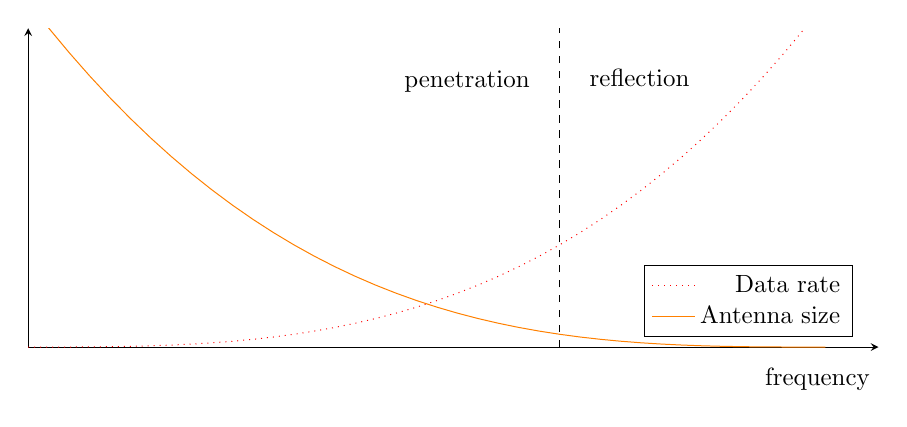
\begin{tikzpicture}[scale=0.9]
\begin{axis}[
x=1.5cm,
y=1.5cm,
axis y line=left,
axis x line=bottom,
xmax=8,xmin=0,
ymin=0,ymax=3,
xlabel=frequency,
x label style={at={(axis description cs:1,-0.1)},anchor=east},
ylabel=,
xmajorticks=false,
ymajorticks=false,
width=15cm,
anchor=center,
legend pos=south east,
legend cell align={right}
]
\addplot+ [samples = 40, domain=0:7.5, no markers, red, dotted] {x^3/130};
\addlegendentry{Data rate}
\addplot+ [samples = 40, domain=0:7.5, no markers, orange] {-(x-7.5)^3/130};
\addlegendentry{Antenna size}
\addplot+ [mark=none, black, dashed] coordinates {(5, 0) (5, 3)};
\node [anchor=east] at (4.8,2.5) {penetration};
\node [anchor=west] at (5.2,2.535) {reflection};
\end{axis}
\end{tikzpicture}
\captionof{figure}{Operation frequencies}
\end{center}

\subsection{Communication, Coding and Modulation}
\begin{mytitle}[Communication principles] The field of the reader may be turned off periodically to allow transponders to send in-between. This requires a capacitor on the transponders to buffer energy.
\end{mytitle}
\begin{mytitle}[Typical encoding schemes] 
    \begin{mysubtitle}[NRZ] 1 = high, 0 = low
    \end{mysubtitle}
    \begin{mysubtitle}[Manchester] 1 = high$\to$low, 0 = low$\to$high. This is typically used for tag to reader communication.
    \end{mysubtitle}
    \begin{mysubtitle}[Pulse pause coding (PPC)] 1 = short period to next pause, 0 = long period to next pause. This is typically used for reader to tag communication.
    \end{mysubtitle}
\end{mytitle}

\subsection{Anti-Collision Protocols}
\begin{mytitle}[The collision problem] The reader broadcasts energy and its signal to many transponders, then all transponders may react simultaneously. They will interfere if there is only a single shared channel. Ideally a transponder should have exclusive access to the shared channel during the short period where it transmits a few bytes. But transponders usually don't hear the signal from other transponders, only the one from the reader. We want access control and collision detection/avoidance to be fast and reliable.
\end{mytitle}
\begin{mytitle}[Collision avoidance with FDMA] This approach needs many channels in parallel, hence it is only suitable for some particular applications with a small, fixed number of transponders.
\end{mytitle}
\begin{mytitle}[Stochastic protocols] Stochastic protocols usually do not detect all tags in one read cycle, there is overall less reader to tag communication and there is typically an ALOHA-based anti-collision algorithm.
    \begin{mysubtitle}[ALOHA principle] Transponders repeatedly send out their data with random length quiet periods in-between. The data should eventually get through. The higher the load, the more collisions happen. This has a maximal throughput of 18.4\%.
    \end{mysubtitle}
    \begin{mysubtitle}[Slotted ALOHA] Transponders start their transmissions only at well-defined instants (slots). Synchronization is done by the reader who periodically sends out "sync" commands. All transponders then send their serial number in one of the following slots. If the reader gets only one serial number "sn", it sends a "select sn" command. Only the transponder with serial number "sn" responds by sending its payload data. The maximal throughput is then 36.8\%. 
    \end{mysubtitle}
    \begin{mysubtitle}[Reservation ALOHA] This protocol has two phases: first a short ALOHA phase where the transponders compete for reservations, then the reserved phase for payload data transmission. 
    \end{mysubtitle}
    \begin{mysubtitle}[Adaptive round algorithm] In this extension of reservation ALOHA the number of slots is dynamically altered, depending on the number of collisions and empty slots.
    \end{mysubtitle}
\end{mytitle}
\begin{center}
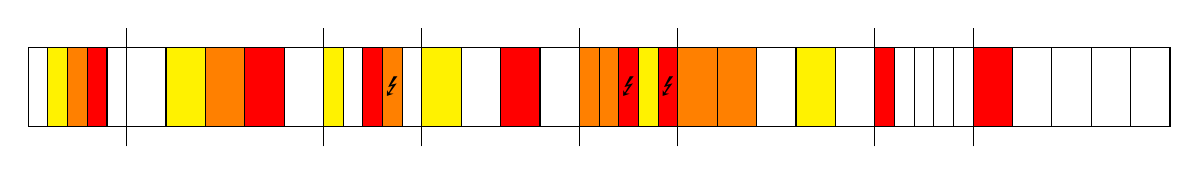
\begin{tikzpicture}[scale = 0.5]

%\draw (0, 0) rectangle (30, 2);
\draw [fill = white] (0, 0) rectangle (0.5, 2);
\draw [fill = yellow] (0.5, 0) rectangle (1, 2);
\draw [fill = orange] (1, 0) rectangle (1.5, 2);
\draw [fill = red] (1.5, 0) rectangle (2, 2);
\draw [fill = white] (2, 0) rectangle (2.5, 2);

\draw [] (2.5, -0.5) -- (2.5, 2.5);

\draw [fill = white] (2.5, 0) rectangle (3.5, 2);
\draw [fill = yellow] (3.5, 0) rectangle (4.5, 2);
\draw [fill = orange] (4.5, 0) rectangle (5.5, 2);
\draw [fill = red] (5.5, 0) rectangle (6.5, 2);
\draw [fill = white] (6.5, 0) rectangle (7.5, 2);

\draw [] (7.5, -0.5) -- (7.5, 2.5);

\draw [fill = yellow] (7.5, 0) rectangle (8, 2);
\draw [fill = white] (8, 0) rectangle (8.5, 2);
\draw [fill = red] (8.5, 0) rectangle (9, 2);
\draw [fill = orange] (9, 0) rectangle (9.5, 2) node[midway] {\Lightning}; 
\draw [fill = white] (9.5, 0) rectangle (10, 2);

\draw [] (10, -0.5) -- (10, 2.5);

\draw [fill = yellow] (10, 0) rectangle (11, 2);
\draw [fill = white] (11, 0) rectangle (12, 2);
\draw [fill = red] (12, 0) rectangle (13, 2);
\draw [fill = white] (13, 0) rectangle (14, 2);
\draw [fill = white] (14, 0) rectangle (15, 2);

\draw [] (14, -0.5) -- (14, 2.5);

\draw [fill = orange] (14, 0) rectangle (14.5, 2);
\draw [fill = orange] (14.5, 0) rectangle (15, 2);
\draw [fill = red] (15, 0) rectangle (15.5, 2) node[midway] {\Lightning}; 
\draw [fill = yellow] (15.5, 0) rectangle (16, 2);
\draw [fill = red] (16, 0) rectangle (16.5, 2) node[midway] {\Lightning}; 

\draw [] (16.5, -0.5) -- (16.5, 2.5);

\draw [fill = orange] (16.5, 0) rectangle (17.5, 2);
\draw [fill = orange] (17.5, 0) rectangle (18.5, 2);
\draw [fill = white] (18.5, 0) rectangle (19.5, 2);
\draw [fill = yellow] (19.5, 0) rectangle (20.5, 2);
\draw [fill = white] (20.5, 0) rectangle (21.5, 2);

\draw [] (21.5, -0.5) -- (21.5, 2.5);

\draw [fill = red] (21.5, 0) rectangle (22, 2);
\draw [fill = white] (22, 0) rectangle (22.5, 2);
\draw [fill = white] (22.5, 0) rectangle (23, 2);
\draw [fill = white] (23, 0) rectangle (23.5, 2);
\draw [fill = white] (23.5, 0) rectangle (24, 2);

\draw [] (24, -0.5) -- (24, 2.5);

\draw [fill = red] (24, 0) rectangle (25, 2);
\draw [fill = white] (25, 0) rectangle (26, 2);
\draw [fill = white] (26, 0) rectangle (27, 2);
\draw [fill = white] (27, 0) rectangle (28, 2);
\draw [fill = white] (28, 0) rectangle (29, 2);

\end{tikzpicture}
\captionof{figure}{Reservation ALOHA}
\end{center}
\begin{mytitle}[Deterministic protocols] Deterministic protocols usually detect all tags that are present in a read cycle, but they introduce high reader to tag communication overheads. There is typically a tree-walking anti-collision algorithm.
    \begin{mysubtitle}[Tree-walking anti-collision algorithm] \hfill
    \begin{itemize}
        \item The coding scheme: We use Manchester encoding, so that where two signals that are transmitting over each other differ, it results in an illegal signal and the reader can locate these bits.
        \item The basic idea: The reader broadcasts a "sync" to all transponders, then requests the ID number of all transponders. It then determines the leftmost bit $b$ that yields a collision. If there is none, the reader requests data from the unique transponder $x$, then sends "halt" to $x$. Then the reader moves up the tree to the next appropriate subtree with a different value of the last $b$. If there is a collision, the reader broadcasts "mute if value 0 at position $b$". Only transponders with value 1 at position $b$ move to the next round, all others remain mute from now on.
    \end{itemize}
    \end{mysubtitle}
\end{mytitle}
\begin{mytitle}[Business-relevant and application-driven criteria] \hfill
\begin{itemize}
    \item Read range: Low and high frequency have a read range of 1-1.5 m, ultra high frequency has a read range of around 10 m. The working area is typically complex.
    \item Data transfer and detection rate: Low and high frequency have a data transfer rate of 5 kb/s, ultra high frequency has a data transfer rate of 50 kb/s. The detection rate depends on the data transfer rate, the choice of anti-collision algorithm and the length of the tag ID. Typically low and high frequency have a detection rate of 10-30 tags/s, ultra high frequency has a range of 100-500 tags/s.
    \item Susceptibility to noise and other error sources: This depends on frequency, antenna size and protocol.
    \item Cost: The cost typically ranges from a few cents to a few dollars.
    \item Form factors: This includes things like the coice of paper vs. plastic.
\end{itemize}
\end{mytitle}

\subsection{Strengths and Drawbacks of RFID}
\begin{mytitle}[Strengths of RFID] \hfill
\begin{itemize}
    \item No line of sight required
    \item Longer read range
    \item More bits
    \item Multiple tags can be read nearly simultaneously
    \item Write and change data
    \item Possibility to integrate sensors
\end{itemize}
\end{mytitle}
\begin{mytitle}[Drawbacks of RFID]\hfill
\begin{itemize}
    \item Cost
    \item Unreliable under certain conditions
\end{itemize}
\end{mytitle}

\section{Smart Cards}
\begin{mytitle}[Main use] Smart cards are portable secure containers for secret data. They are a secure environment for cryptographic algorithms, but they are also interesting for ubicomp technology because they are a cheap, small and disposable computer with security tokens. 
\end{mytitle}
\begin{mytitle}[Memory cards vs processor cards] Memory cards are just a container for data, usually with access control for parts of the memory. They are cheap but not truly smart. Processor cards on the other hand have an internal microprocessor and RAM. They optionally contain a true random generator or hardware crypt-functionality.
\end{mytitle}
\begin{mytitle}[Communication with the card] Communication between the card reader and the smart card is always initiated by the reader. The card gets Vcc and CLK and does a "reset". Within a few ms, it sends back an "answer to reset" (ATR) containing basic information about the card. Then the terminal sends the first command application protocol data unit (APDU) to the card and the card answers with a response APDU. Encryption and authentication is possible, but slows down the communication by a factor of 4.
\end{mytitle}
\begin{mytitle}[Subscriber identity module (SIM)] The SIM is the security module for accessing the mobile phone network.
\end{mytitle}
\begin{mytitle}[Contact-less smart cards] These smart cards use an external energy source like RFID does. They are more expensive but have better security compared to RFID tags.
\end{mytitle}
\begin{myremark} The secret data inside the card must never leave the card and computations must not be observable from the outside.
\end{myremark}
\begin{mytitle}[Entity authentication] The terminal verifies the card (internal auth) and the card verifies the terminal (external auth). Then the terminal asks the user to provide the password and sends it to the card for verification.
\end{mytitle}

\subsection{Attacks}
\begin{mytitle}[Attack classification] There are three kinds of attackers:
\begin{itemize}
    \item Clever outsiders: they use existing weaknesses in systems
    \item Knowledgeable insiders: they have access to highly sophisticated tools
    \item Funded organizations: they have virtually unlimited resources
\end{itemize}
\end{mytitle}
\begin{mytitle}[Leakage] Power consumption, heat, electromagnetic emissions, timing and faulty outputs are all side-channel informations that get leaked and can be used in attacks.
\end{mytitle}
\begin{mytitle}[Simple attacks]\hfill
\begin{itemize}
    \item Clock bursts: momentarily cause a rapid increase in the clock frequency, this causes instructions to be skipped
    \item Voltage glitch: momentarily cause a drop in voltage, this causes instructions to be decoded incorrectly
    \item Acid hacking: gain access to ROM by physically looking at it to see the bits
\end{itemize}
\end{mytitle}
\begin{mytitle}[More advanced attacks]\hfill
\begin{itemize}
    \item Power analysis attack: The attacker measures the power consumption to learn the bits of the secret key. When no special counter-measures are taken, this is applicable for almost all crypt-algorithms and smart cards.
    \item Hamming weight leakage: The attacker learns the number of 1s in each of the seven 8-bit words of the secret key. This reduces the brute-force search space from $2^{56}$ to $2^{40}$.
    \item Timing attack: Because there is code that is only executed when the bit is 1, the operation will take a bit longer in that case. From this information the attacker can also learn the bits of the secret key.
\end{itemize}
\end{mytitle}

\subsection{Counter-measures}
\begin{mytitle}[Hardware counter-measures] \hfill
\begin{itemize}
    \item Balance/equalize power consumption
    \item Increase noise
    \item Vary the execution time of instructions
    \item Randomly modify the internal clock speed
\end{itemize}
\end{mytitle}
\begin{mytitle}[Software counter-measures]\hfill
\begin{itemize}
    \item Add random instructions to desynchronize
    \item Don't let the timing depend on the data or the key
    \item Limit the number of times an algorithm can be executed
\end{itemize}
\end{mytitle}
\begin{mytitle}[General counter-measures]\hfill
\begin{itemize}
    \item Scramble the data bus and memory cells/addresses differently for each chip
    \item Use dual logic where 10 = low and 01 = high. They always consume the same amount of power.
    \item Use a dual CPU where the same operation is performed on two CPUs and then compared.
    \item Use checksums on memory content.
    \item Encrypt the memory content
    \item Encrypt/decrypt the data on the bus with dynamic random keys.
    \item Use shielding and protection layers
\end{itemize}
\end{mytitle}
\begin{mytitle}[Active hardware counter-measures]\hfill
\begin{itemize}
    \item Use sensors reacting to light, temperature sensors against increased clock rates and resistance/capacity sensors to detect removal of the chips protection layers.
    \item Watch the current and clock-frequency to detect hardware attacks.
    \item Do functional tests of parts of the chip.
    \item Overwrite critical parts of the EEPROM when an attack is suspected.
    \item Coat the chip with ransom particles with a high dielectric constant. An array of capacitive sensors detects those properties and uses them as secret random information
\end{itemize}
\end{mytitle}
\section{Establishing Connectivity}
\begin{mytitle}[How to connect UbiComp functionality?] We can connect on three levels: on the physical and medium access layer via low-power wireless, on the network level via internet of things (IoT) and on the application layer via web of things (WoT).
\end{mytitle}

\subsection{Low-Power Wireless}
\begin{mytitle}[Wireless communication]
    \begin{mysubtitle}[Wireless communication benefits]\hfill
    \begin{itemize}
        \item Supports mobility
        \item Less infrastructure
    \end{itemize}
    \end{mysubtitle}
    \begin{mysubtitle}[Wireless communication drawbacks]\hfill
    \begin{itemize}
        \item Typically lower transmission rates
        \item Restrictive regulation of resources
        \item Lower security
        \item Higher loss rates
        \item Higher power consumption
    \end{itemize}
    \end{mysubtitle}
\end{mytitle}
\begin{mytitle}[Energy harvesting] We can harvest power directly from switching events. A spring in a switch outputs enough energy to transmit three identification messages. Other sources of energy include wrist-watches, photovoltaic, piezoelectricity, pyroelectricity, atmospheric pressure changes and other ambient radiation.
\end{mytitle}
\begin{mytitle}[Wi-Fi (802.11)] Wi-Fi is a power-consuming communication system, therefore there is no wide adaptation in the sensor network and IoT space. Instead they rely on 802.15.4 (a standard for low-rate WPANs) and bluetooth low energy (BLE).
\end{mytitle}
\begin{mytitle}[Passive Wi-Fi] Passive Wi-Fi uses backscatter communication to generate up to 11 Mbit/s transmissions and has 3-4 orders of magnitude lower energy consumption. It works by offloading RF componenets to a single plugged-in device in the network, creating a single-frequency tone. Passive Wi-Fi devices communicate by reflecting this tone via a digital switch. Those transmissions can be decoded by all devices within a Wi-Fi chipset. The range is typically 10-100 m.
\end{mytitle}
\begin{mytitle}[Interscatter] Interscatter describes the modulation of the reflection of a BLE packet to generate a Wi-Fi packet.
\end{mytitle}
\begin{mytitle}[Ultra-low-power communication] The core idea is to exploit energy asymmetries. Every sensor node has very little power but there is a sink node with lots of power.
    \begin{mysubtitle}[Low-power listening (LPL)] Receivers periodically wake up to sample the wireless channel to detect activity from the sender.
    \end{mysubtitle}
    \begin{mysubtitle}[Low-power probing (LPP)] Receivers periodically wake up and send probes and go back to sleep after a short amount of time. The sender listens for probes and sends the payload immediately after receiving one.
    \end{mysubtitle}
\end{mytitle}
\begin{mytitle}[Multiplexing] The goal here is to make best use of the precious shared wireless medium.
    \begin{mysubtitle}[Space division mutltiple access (SDMA)] Here we segment space into cells/sectors. We use the same frequencies in different cells. The advantage is its simplicity. The disadvantages are the needed infrastructure investment and handover management.
    \end{mysubtitle}
    \begin{mysubtitle}[Frequency division multiple access (FDMA)] Here we separate the spectrum into smaller frequency bands and allocate one band per channel. The advantage is that there is no need for co-ordination. The disadvantages are the possible waste of bandwidth and its inflexibility.
    \end{mysubtitle}
    \begin{mysubtitle}[Time division multiple access (TDMA)] Here one channel gets the entire spectrum but only for a short period of time. The advantages are that we use only one carrier at at time and that there is higher throughput possible. The disadvantage is the precise synchronization that is needed.
    \end{mysubtitle}
    \begin{mysubtitle}[Combination of FDMA + TDMA (+ SDMA)] A combination has the advantages that it is more robust against selective interference and has better eavesdrop resistance. The disadvantage is the precise synchronization that is needed.
    \end{mysubtitle}
    \begin{mysubtitle}[Code division multiple access (CDMA)] Here we take a narrowband signal and spread it over the available spectrum. All channels then use the same spectrum simultaneously and statistical methods are used to disentangle the signals. Each channel has a unique code. In DS-CDMA the code is used to chip the signal into smaller pieces, while in FH-CDMA the code is used as a hopping pattern between frequencies. The advantages here are its bandwidth efficiency, that no synchronization is needed and its robustness against interference and eavesdropping. The disadvantage is that more complex signal filtering is needed for decoding the signals.
    \end{mysubtitle}
\end{mytitle}
\begin{mytitle}[Low-power wide area network (LPWAN)] We want long range, a low number of base stations, a low data rate, low battery and low subscription costs. Examples of LPWAN providers are SigFox and LoRa.
\end{mytitle}

\subsection{Bluetooth}
\begin{mytitle}[Bluetooth] Bluetooth is intended as a WLAN replacement in personal area networks. It is much smaller, cheaper and needs less power, but only has a short range ($\sim$10 m) and up to 720 kb/s. It also needs a complex communication stack to support voice and data as well as bluetooth profiles for different device functions. 
\end{mytitle}
\begin{center}
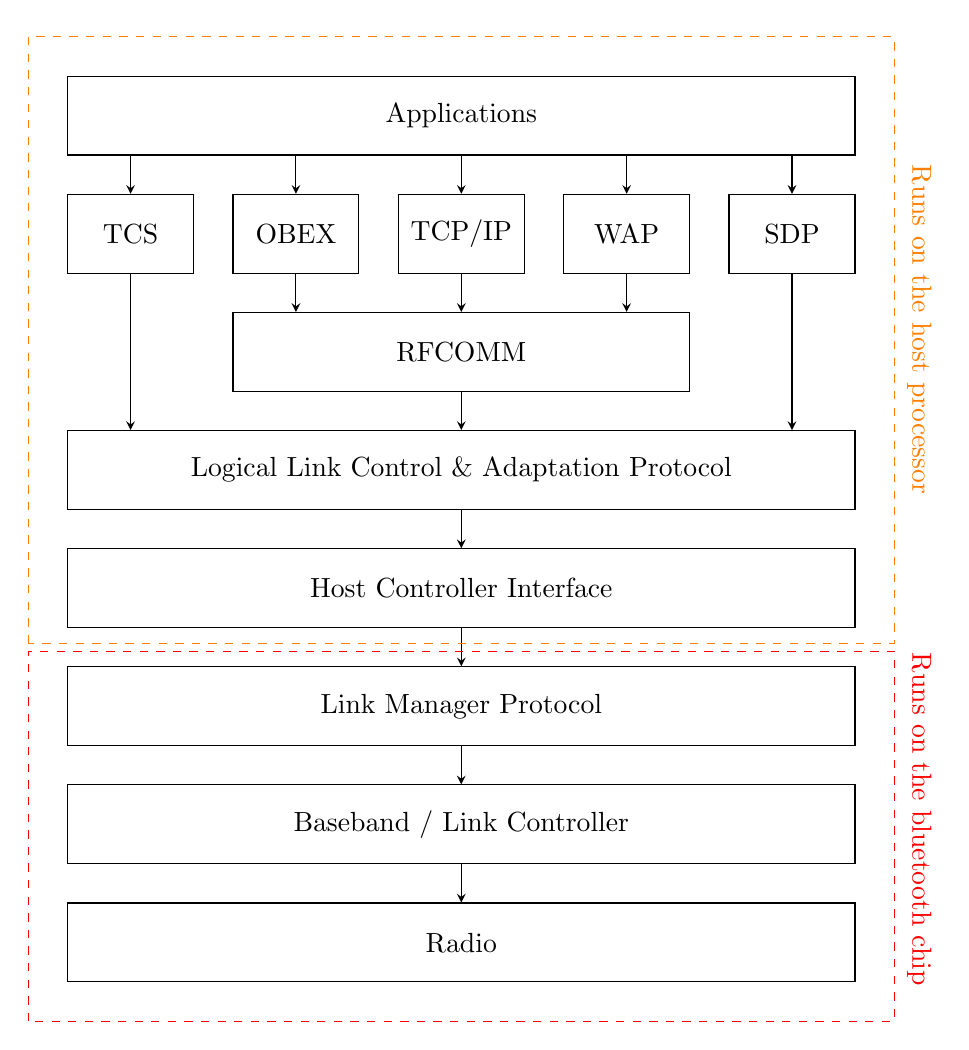
\begin{tikzpicture}

\node (A) at (5,-1) [draw,minimum width=10cm,minimum height=1cm] {Radio};
\node (B) at (5,0.5) [draw,minimum width=10cm,minimum height=1cm] {Baseband / Link Controller};
\node (C) at (5,2) [draw,minimum width=10cm,minimum height=1cm] {Link Manager Protocol};
\node (D) at (5,3.5) [draw,minimum width=10cm,minimum height=1cm] {Host Controller Interface};
\node (E) at (5,5) [draw,minimum width=10cm,minimum height=1cm] {Logical Link Control \& Adaptation Protocol};
\node (F) at (5,6.5) [draw,minimum width=5.8cm,minimum height=1cm] {RFCOMM};
\node (G1) at (0.8,8) [draw,minimum width=1.6cm,minimum height=1cm] {TCS};
\node (G2) at (2.9,8) [draw,minimum width=1.6cm,minimum height=1cm] {OBEX};
\node (G3) at (5,8) [draw,minimum width=1.6cm,minimum height=1cm] {TCP/IP};
\node (G4) at (7.1,8) [draw,minimum width=1.6cm,minimum height=1cm] {WAP};
\node (G5) at (9.2,8) [draw,minimum width=1.6cm,minimum height=1cm] {SDP};
\node (H) at (5, 9.5) [draw,minimum width=10cm,minimum height=1cm] {Applications};

\draw [->] (G1 |- H.south) -- (G1);
\draw [->] (G2 |- H.south) -- (G2);
\draw [->] (G3 |- H.south) -- (G3);
\draw [->] (G4 |- H.south) -- (G4);
\draw [->] (G5 |- H.south) -- (G5);
\draw [->] (G1.south) -- (G1 |- E.north);
\draw [->] (G2.south) -- (G2 |- F.north);
\draw [->] (G3.south) -- (G3 |- F.north);
\draw [->] (G4.south) -- (G4 |- F.north);
\draw [->] (G5.south) -- (G5 |- E.north);
\draw [->] (F) -- (E);
\draw [->] (E) -- (D);
\draw [->] (D) -- (C);
\draw [->] (C) -- (B);
\draw [->] (B) -- (A);

\draw [dashed, firstAccent] (-0.5, 2.8) rectangle (10.5, 10.5) node [label={[label distance=1.5cm,text depth=3ex,rotate=-90, firstAccent]right:Runs on the host processor}] {};
\draw [dashed, secondAccent] (-0.5, -2) rectangle (10.5, 2.7) node [label={[label distance=-0.1cm,text depth=3ex,rotate=-90, secondAccent]right:Runs on the bluetooth chip}] {};

\end{tikzpicture}
\captionof{figure}{Classic Bluetooth protocol stack}
\end{center}
\newpage
\begin{mytitle}[Frequency hopping on the radio layer] If a collision occurs, a packet is retransmitted on a different channel. The specific hopping pattern is not known to outsiders. A common hopping sequence for all cooperating devices is determined by the baseband layer. There are about 1600 hops/s.
\end{mytitle}
\begin{mytitle}[Baseband]
    \begin{mysubtitle}[Addressing] Each bluetooth device has a 48 bit device ID. There is a 3 bit active member address (AMA) when it is active in a piconet and an 8 bit parked member address (PMA) when it is not active. A piconet consists of bluetooth units sharing a single frequency-hopping channel. A single master connects to a maximum of 7 slaves due to the 3 bit address. Communication is point-to-point master-slave or multicast from the master to all of its slaves.
    \end{mysubtitle}
    \begin{mysubtitle}[Connection states] There are 7 different states:
    \begin{itemize}
        \item Standby: not participating in a piconet
        \item Inquiry: learn about identity of other devices around
        \item Page: invitation to a known device to join
        \item Active: full power mode, listening to all packets
        \item Sniff: low power mode, wakes up every x ms to check
        \item Park: low power mode, only listens to sync beacons, not used anymore
        \item Hold: low power mode, master puts device on hold, slave returns automatically
    \end{itemize}
    \begin{center}
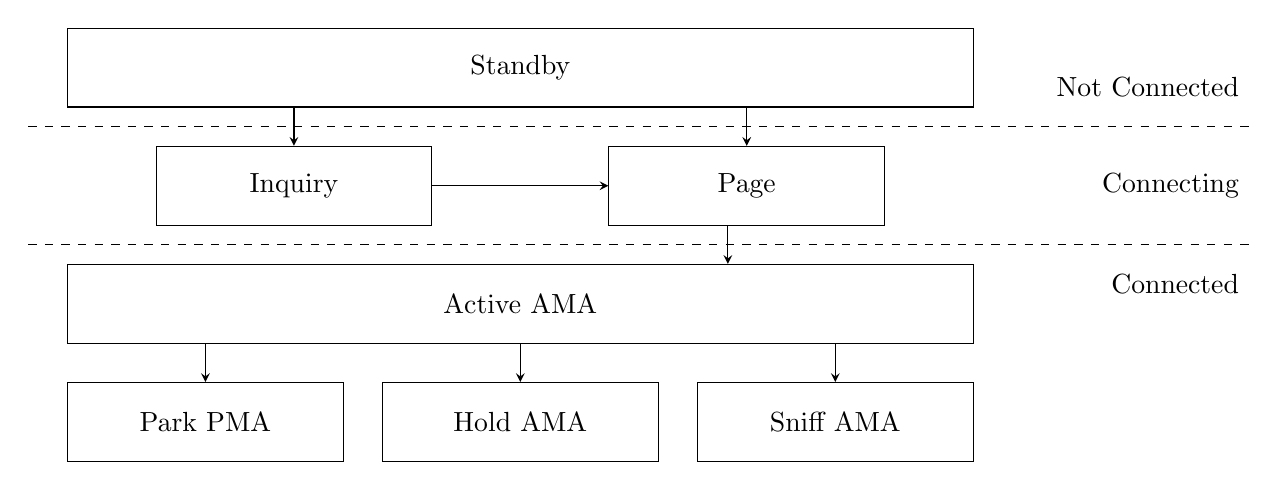
\begin{tikzpicture}

\node (A) at (5.75,4.5) [draw,minimum width=11.5cm,minimum height=1cm] {Standby};
\node (B1) at (2.875,3) [draw,minimum width=3.5cm,minimum height=1cm] {Inquiry};
\node (B2) at (8.625,3) [draw,minimum width=3.5cm,minimum height=1cm] {Page};
\node (C) at (5.75,1.5) [draw,minimum width=11.5cm,minimum height=1cm] {Active AMA};
\node (D1) at (1.75,0) [draw,minimum width=3.5cm,minimum height=1cm] {Park PMA};
\node (D2) at (5.75,0) [draw,minimum width=3.5cm,minimum height=1cm] {Hold AMA};
\node (D3) at (9.75,0) [draw,minimum width=3.5cm,minimum height=1cm] {Sniff AMA};

\draw [->] (B1 |- A.south) -- (B1);
\draw [->] (B2 |- A.south) -- (B2);
\draw [->] (B1) -- (B2);
\draw [->] ([xshift=7.5em]C |- B2.south) -- ([xshift=7.5em]C.north);
\draw [->] (D1 |- C.south) -- (D1);
\draw [->] (D2 |- C.south) -- (D2);
\draw [->] (D3 |- C.south) -- (D3);

\draw [dashed] (-0.5,2.25) -- (15,2.25);
\draw [dashed] (-0.5, 3.75) -- (15,3.75);

\node at (15, 4.25) [anchor=east] {Not Connected};
\node at (15, 3) [anchor=east] {Connecting};
\node at (15, 1.75) [anchor=east] {Connected};

\end{tikzpicture}
\captionof{figure}{Baseband Connection States}
\end{center}
    \end{mysubtitle}
    \begin{mysubtitle}[Packet Format] 72 bits access code, 54 bits header, 0-2745 bits payload
    \end{mysubtitle}
    \begin{mysubtitle}[Error Handling]\hfill
    \begin{itemize}
        \item Automatic repeat request (ARQ): If the sender does not receive a 1-bit ACK before the timeout, it usually re-transmits the packet until it receives the ACK or exceeds a predefined number of retransmissions.
        \item Forward error correction (FEC): The sender encodes the message in a redundant way by using an error-correcting code (ECC). This reduces the number of repeat requests but adds overhead.
    \end{itemize}
    \end{mysubtitle}
\end{mytitle}


\begin{mytitle}[Link manager] The link manager manages the piconet, authentication (only accept connections from trusted devices), switching of master/slave roles and the tearing down of connections when slaves leave. It also handles the low power modes. Active voice mode uses around 10 mA, active data mode uses around 6 mA and hold/park mode only 60 $\mu$A. For comparison bluetooth low energy has a 1 $\mu$A average.
\end{mytitle}
\begin{mytitle}[Logical link control \& adaptation protocol (L2CAP)] L2CAP adapts the upper layer protocols to the baseband. It handles the segmentation and reassembly of the upper layer protocol packets and the protocol multiplexing over a single air interface.
\end{mytitle}
\begin{mytitle}[Radio frequency communication (RFCOMM)] RFCOMM emulates a serial port and thus allows multiple ``ports'' over a single bluetooth channel. This enables TCP/IP and roughly the same service and reliability guarantees as TCP.
\end{mytitle}
\begin{mytitle}[Bluetooth low energy (BLE)] BLE has up to 260 Kbps data rate and only sends occasional updates of sensor values. It does not have voice support, has fewer but broader channels, has a faster connection setup and the modulation scheme is optimized for low power usage.
\end{mytitle}
\begin{mytitle}[Generic attribute profile (GATT)] GATT is the BLE application-layer protocol that reads and writes remote variables, the length of which typically ranges between 20 and 40 bytes. Related characteristics are grouped into services (based on GATT) like ``Device information service'', ``Heart rate profile'', etc. The central device is the GATT client while the peripheral devices are GATT servers. Peripheral-peripheral communication is possible through abstractions managed by the central device.
\end{mytitle}
\begin{mytitle}[IPv6-based LPWANs] These want direct end-to-end internet integration of resource-constrained embedded devices. Edge routers are used to connect the LoWPAN to the IP infrastructure. An example provider is 6LoWPAN, which transports IPv6 packets over BLE while recognizing and implementing BLE's limits on protocol overhead. A border router connects LWPANs to IP infrastructure, performs (de-)compression and disseminates routing information.
\end{mytitle}

\subsection{Internet of Things}
\begin{mytitle}[Transmission control protocol (TCP)] TCP establishes connectivity between processes. 
    \begin{mysubtitle}[Three-way handshake] SYN, SYN-ACK, ACK
    \end{mysubtitle}
    \begin{mysubtitle}[Sequence number and ack number] These numbers enable the in-order delivery of packets
    \end{mysubtitle}
    \begin{mysubtitle}[Window] Windows are the limit on packets that can be ``in flight'' simultaneously
    \end{mysubtitle}
    \begin{mysubtitle}[Flow control] Flow control makes sure that networks are not overloaded. AIMD is the classic flow control implementation.
    \end{mysubtitle}
\end{mytitle}
\begin{mytitle}[User datagram protocol (UDP)] UDP is used by applications that do not require the reliability of TCP. It is much more leightweight as there is no connection setup and little overhead.
\end{mytitle}
\begin{mytitle}[Representational state transfer (REST)] REST provides architectural guidelines for computing infrastructure, including the web. It is a resource-oriented architecture (ROA), meaning that the functionality is integrated into resources, not offered by services. 
\end{mytitle}
\begin{mytitle}[REST Constraints] REST defines 6 architectural constraints which make any web service a true RESTful API. 
    \begin{mysubtitle} [Uniform interface] You must decide the APIs interface for resources inside the system which are exposed to the API consumers and follow it religiously. A resource in the system should have only one logical URI and that should provide a way to fetch related or additional data.
    \end{mysubtitle}
    \begin{mysubtitle} [Client-Server] The client application and server application must be able to evolve separately without any dependency on each other. A client should know only resource URIs and that’s all. 
    \end{mysubtitle}
    \begin{mysubtitle} [Stateless] All client-server interaction are stateless. The server will not store anything about the latest HTTP request a client made but will treat each and every request as new.
    \end{mysubtitle}
    \begin{mysubtitle} [Cacheable] Caching shall be applied to resources when applicable and then these resources must declare themselves cacheable. Caching can be implemented on the server or client side.
    \end{mysubtitle}
    \begin{mysubtitle} [Layered system] REST allows you to use a layered system architecture where you deploy the APIs on server A, and store data on server B and authenticate requests in Server C, for example. A client cannot ordinarily tell whether it is connected directly to the end server, or to an intermediary along the way.
    \end{mysubtitle}
    \begin{mysubtitle} [Code on demand (optional)] When you need to, you are free to return executable code to support a part of your application e.g. clients may call your API to get a UI widget rendering code.
    \end{mysubtitle}
\end{mytitle}
\begin{myremark} In REST, there is state in resources and in the client, but not in the transaction. This enables that a series of interactions by a client can be handled by different servers.
\end{myremark}
\begin{mytitle}[Web resources] A web resource is ``anything that you want to talk about'', like products, categories, customers, shopping carts, etc. but also client state transitions like next links and paged results.
\end{mytitle}
\begin{myremark} In HTTP, verbs stay polymorphic, i.e. we use GET for all types of resources. In contrast RPC-style WS$^*$-web services define operations specific for object types.
\end{myremark}
\begin{mytitle}[Shared representation model]Every web browser can access every web resource because HTTP works the same for every resource. Interacting with the resource is possible without knowing it beforehand. The representations that are exchanged depend on a shared representation model.
\end{mytitle} 
\begin{mytitle}[Resource representations] Resources are abstract entities, interaction with resources happens via resource representations. Representation formats can be negotiated between peers and it is communicated which kind of representation is used. When you access a web resource, you see one of its representations your browser negotiates for you. Resource representations contain links to identified resources. Servers guide interactions by providing links. Links are possible state transitions of the client/server application.
\end{mytitle}

\subsection{Web of Things}
\begin{mytitle}[IoT vs WoT] IoT describes the global network of physical objects that communicate using the internet protocol. WoT refers to a specific part of the WWW where physical entities are identified by URLs and interlinked by hyperlinks.
\end{mytitle}
\begin{mytitle}[Hypermedia as the engine of application state (HATEOAS)] With HATEOAS, a machine API needs no syntactic documentation. Making full use of the WoT (including HATEOAS) for devices and services facilitates the autonomous usage of their interface by machine clients and the creation of flexible mashups across services by different providers. HATEOAS makes systems flexible and robust by decoupling clients and servers as clients discover state transitions at runtime.
\end{mytitle}
\begin{mytitle}[HTTP] HTTP is a text-based protocol. HTTP requests indicate the action to be performed and what type of response the client will accept. The advantages are that it is understandable and debuggable. The disadvantage is that it is not very efficient. 
\end{mytitle}
\begin{mytitle}[The constrained application protocol (CoAP)] CoAP is an alternative to HTTP, targeted to constrained nodes and networks. Constrained nodes can be sensors with limited memory and processing power and constrained networks can be slow, unreliable and intermittent. CoAP is optimized for bandwidth and processing efficiency. It is based on UDP and has lightweight security. In CoAP, the client can send an observe to the server, then it will get notifications about resource state changes. There also exists support for multicast. Security in CoAP emulates a 3-way handshake. For low-power devices there is still ongoing work.
    \begin{mysubtitle}[Message types] There are four message types in CoAP:
    \begin{itemize}
        \item Confirmable (CON): reliable message with retransmission
        \item Non-Confirmable (NON): best effort transmission
        \item Acknowledgement (ACK): confirms a CON message
        \item Reset (RST): used when CON or NON cannot be processed
    \end{itemize}
    CONs retransmit after 2-3 seconds. The timeout is doubled after each retransmission. Retransmissions stop when an ACK arrives or after 4 retransmissions failed. CONs and ACKs are matched through the message ID (MID).
    \end{mysubtitle}
\end{mytitle}

\input{7_location.tex}
\section{Societal Implications}
\begin{mytitle}[Nudging] Nudging is a mild and more accepted version of paternalism.
\end{mytitle}
\begin{mytitle}[Relevant technological development]\hfill
\begin{itemize}
    \item Computer vision: recognizing objects, situations, people, etc.
    \item Artificial intelligence: smart/autonomous systems, self-driving cars, etc.
    \item Wearable computing: components are distributed over the body and in clothes. They acquire context data and augment the users view of the envrionment. They have a hands free, intuitive user interface.
    \item Augmented reality: providing context information, intuitive interfaces, etc.
\end{itemize}
\end{mytitle}
\begin{mytitle}[Hybrid products] Hybrid products are physical items together with an added value provided by embedded ICT. They provide the user with a wealth of background information. The device is sold together with a service which makes it more difficult to imitate.
\end{mytitle}
\begin{mytitle}[New business opportunities] Tasks that could not be monitored can now be measured, controlled, managed and priced using embedded sensors and wireless feedback. We can measure the usage of a product or a service and then pay per use. Possible effects are more efficient markets, fairer prices, more adequate supply and better utilization of resources but also more stress for the consumer.
\end{mytitle}
\begin{mytitle}[Social risks] Social risks include smart things that may behave unexpectedly, self-determination, incresed dependability and privacy concerns.
\end{mytitle}
\section{Economical Aspects}
\begin{mytitle}[Servitization] Servitization defines the departure from just producing physical goods towards a combination of physical goods and services. The desired continued economic sutainability (market pull) and technological innovation (technology push) drive servitization through digitalization. Because there is a large "installed base" and there are usually higher margins in the service business, there is an economic incentive to shift to aftermarket services.
\end{mytitle}
\begin{mytitle}[Risk and drawbacks]
    \begin{mysubtitle}[Risks for service providers] Risks include erosion of economics of scale, availability is king thus penalty clauses directly impact profitability, the temptation to be too ambitious with promises and that the promises to the customers might require additional resources.
    \end{mysubtitle}
    \begin{mysubtitle}[Risks for customers] Risks include the product/ecosystem lock-in and no legal ownership of the product means there are constraints on the own operations.
    \end{mysubtitle}
\end{mytitle}
\renewcommand{\arraystretch}{2}
\begin{center}
\begin{tabu} to 0.9\textwidth {  l | X[l] | X[l]  }
& Technology push & Market pull \\
\hline
Sense & New sensor technologies & Necessary to understand own products performance and cost\\
Connect & New communication technologies & Necessary to ship this data to back end\\
Analyze & New methods to acquire and process large amounts of data & Necessary to react fast to malfunctions or better forecast them\\
Control & New materials and softwareization & Even better to upgrade products remotely\\
Integrate & New architecures/infrastructures to integrate services & Products and services need to be flexible and future-proof
\end{tabu}
\captionof{table}{Technological push and market pull}
\end{center}
\begin{mytitle}[High-resolution management] The goal is to support management tasks like planning, leadership and controlling with automated data collection. This also means that digital business model patterns are becoming relevant to physical industries for the first time. 
\end{mytitle}
\begin{myremark} Traditionally information is not defined and is expected to be free of charge. The IoT business model sees information as a major source for value in the IoT.
\end{myremark}
\begin{mytitle}[New business model patterns]\hfill
\begin{itemize}
    \item Physical freemium: Sell asset together with a free digital service but premium services are available.
    \item Digital add-on: Sell asset very inexpensively but customers can purchase higher-margin digital services. Invite third parties to sell add-ons as well.
    \item Digital lock-in: Limit the product compatibility to prevent counterfeits and ensure warranty.
    \item Product as point-of-sales: Product takes on a marketing/sales role.
    \item Object self-service: Smart items that place orders on the internet themselves.
\end{itemize}
\end{mytitle}

\end{document}
